% =============================================================================
% Section 16: Embedded Implementation
% =============================================================================

\subsection{Embedded Preliminary Implementation}
\label{sec:embedded_impl}
\sectionauthors{BS, JH}

This section covers embedded systems architecture, communication protocols, and motor control implementation. See Section~\ref{sec:electrical_impl} for hardware specifications and schematics.

\subsubsection{System Architecture Overview}

The distributed architecture separates high-level processing from real-time control:

\begin{figure}[H]
\centering
\resizebox{\textwidth}{!}{%
\begin{tikzpicture}[
    node distance=1cm,
    block/.style={rectangle, draw, rounded corners, minimum width=2.5cm, minimum height=1cm, align=center, font=\small},
    arrow/.style={->, thick, >=stealth}
]
    % Main nodes
    \node[block, fill=blue!20] (pi5) {Raspberry Pi 5\\(ROS 2 / Nav2)};
    \node[block, fill=orange!20, right=5cm of pi5] (esp32) {ESP32-S3\\(FreeRTOS)};

    % Peripherals under Pi5 (horizontally arranged)
    \node[block, fill=green!15, below=2cm of pi5, xshift=-5cm] (lidar) {LiDAR\\(SICK/RPLiDAR)};
    \node[block, fill=green!15, right=0.3cm of lidar] (imu) {IMU\\(BNO055)};
    \node[block, fill=green!15, right=0.3cm of imu] (camera) {Stereo\\Camera};
    \node[block, fill=green!15, right=0.3cm of camera] (sonars) {Ultrasonics\\(7x)};

    % Peripherals under ESP32
    \node[block, fill=yellow!20, below=2cm of esp32, xshift=-0.5cm] (drivers) {Motor\\Drivers (4x)};
    \node[block, fill=yellow!20, right=0.3cm of drivers] (temp) {Temp Sensor\\(DS18B20)};
    \node[block, fill=red!15, right=3.5cm of esp32] (bms) {BMS\\(BQ78350)};

    % SPI connection
    \draw[arrow, <->, very thick, blue] (pi5) -- node[above, font=\footnotesize] {SPI @ 10 MHz} (esp32);

    % Pi5 connections
    \draw[arrow] (lidar) -- (pi5);
    \draw[arrow] (imu) -- (pi5);
    \draw[arrow] (camera) -- (pi5);
    \draw[arrow] (sonars) -- (pi5);

    % ESP32 connections
    \draw[arrow, <->] (esp32) -- (drivers);
    \draw[arrow] (temp) -- (esp32);
    \draw[arrow, <->] (esp32) -- node[above, font=\tiny] {SMBus} (bms);

    % Labels
    \node[font=\footnotesize\bfseries, above=0.3cm of pi5] {High-Level (Linux)};
    \node[font=\footnotesize\bfseries, above=0.3cm of esp32] {Real-Time (RTOS)};
\end{tikzpicture}%
}
\caption{Distributed Compute Architecture}
\label{fig:embedded-arch}
\end{figure}

\subsubsection{Communication Protocols}

Three communication buses connect system components:

\begin{table}[H]
\centering
\caption{Communication Bus Summary}
\begin{tabular}{@{}llllp{4cm}@{}}
\toprule
\textbf{Bus} & \textbf{Speed} & \textbf{Controller} & \textbf{Peripheral} & \textbf{Purpose} \\
\midrule
SPI-1 & 10 MHz & Pi 5 & ESP32 & Velocity commands, sensor data \\
SPI-2 & -- & ESP32 & DRV8243 & Motor config, fault status \\
SMBus & 100 kHz & ESP32 & BQ78350 & Battery SOC, alerts \\
1-Wire & -- & ESP32 & DS18B20 & Temperature compensation \\
\bottomrule
\end{tabular}
\end{table}

\paragraph{SPI Bus Configuration}

\begin{table}[H]
\centering
\caption{SPI-1 Pin Mapping (Pi 5 $\leftrightarrow$ ESP32)}
\begin{tabular}{@{}lll@{}}
\toprule
\textbf{Signal} & \textbf{Pi 5 GPIO} & \textbf{ESP32 GPIO} \\
\midrule
COPI (Controller Out) & GPIO11 & GPIO13 \\
CIPO (Controller In) & GPIO9 & GPIO12 \\
SCLK & GPIO11 & GPIO14 \\
CS & GPIO8 & GPIO15 \\
\bottomrule
\end{tabular}
\end{table}

The N16 variant (no PSRAM) frees GPIO 35--37 for SPI-2 to connect to motor drivers. Firmware uses a unified bus abstraction layer for driver interchangeability.

\paragraph{SMBus for Battery Management}

SMBus (vs. I2C) provides BMS-specific features \parencite{smbus_spec, analog_i2c_smbus}:

\begin{table}[H]
\centering
\caption{SMBus Features for BMS}
\begin{tabular}{@{}lp{8cm}@{}}
\toprule
\textbf{Feature} & \textbf{Benefit} \\
\midrule
Mandatory Timeout & 25--35 ms timeout prevents bus lockups \\
Packet Error Check & CRC-8 checksum for noisy environments \\
SMBALERT\# & Interrupt-driven fault notification (OV, OC, thermal) \\
SBS Commands & Standardized SOC, voltage, current, temperature queries \\
\bottomrule
\end{tabular}
\end{table}

\paragraph{Temperature Compensation}

The DS18B20 provides $\pm$0.5$^\circ$C accuracy for ultrasonic speed-of-sound compensation \parencite{ds18b20_datasheet}:
\begin{equation}
v_{sound} = 331.3 + 0.606 \cdot T_{celsius} \textrm{ m/s}
\end{equation}
This improves ultrasonic distance accuracy from $\pm$3\% to $\pm$0.5\%.

\subsubsection{Motor Control Implementation}

The ESP32's MCPWM peripheral drives four DRV8243 H-bridges (see Section~\ref{sec:implementation} for motor/driver specs).

\paragraph{Center-Aligned PWM}

MCPWM uses center-aligned (up-down count) rather than edge-aligned PWM \parencite{esp_idf_mcpwm, ti_pwm_techniques}.

\subparagraph{PWM Fundamentals}
PWM controls motor speed by rapidly switching power on and off. The \textit{duty cycle} (percentage of time the output is HIGH) determines average voltage delivered to the motor. Hardware PWM uses a counter that continuously increments and a compare register holding the duty cycle threshold. When counter $<$ threshold, output is HIGH; when counter $\geq$ threshold, output is LOW.

\subparagraph{Edge-Aligned vs. Center-Aligned}
The key difference is how the counter behaves. Each motor has a different duty cycle at any given moment (one motor might be at 25\%, another at 75\%, depending on how the robot is turning). The comparison rule is: output = HIGH when counter $<$ threshold.

\textbf{Edge-aligned (sawtooth):} Counter counts from 0 to MAX, then instantly resets to 0. When the counter resets, it goes below \textit{all} thresholds simultaneously, causing all outputs to go HIGH at the same instant. Both motors turn ON at reset, creating a current spike.

\textbf{Center-aligned (triangle):} Counter counts from 0 to MAX, then back down to 0. There is no instant reset. The output toggles twice per cycle (once on the way up, once on the way down), and since each motor has a different threshold, they cross at different times.

Figure~\ref{fig:pwm-comparison} illustrates this with two motors at 25\% and 75\% duty cycles. Edge-aligned bunches two transitions at reset (current spike), while center-aligned spreads four transitions across the entire cycle.

\begin{figure}[H]
\centering
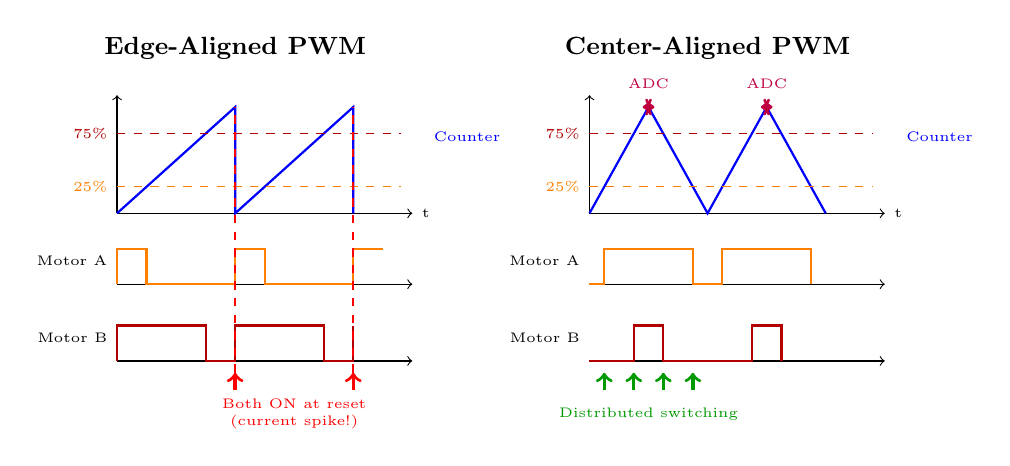
\begin{tikzpicture}[scale=0.75]
    % ===== EDGE-ALIGNED PWM (left side) =====
    \begin{scope}[xshift=-6.5cm]
        \node[font=\small\bfseries] at (2, 5) {Edge-Aligned PWM};

        % Timer counter (sawtooth)
        \draw[->] (0, 2.2) -- (5, 2.2) node[right, font=\tiny] {t};
        \draw[->] (0, 2.2) -- (0, 4.2);
        \draw[thick, blue] (0, 2.2) -- (2, 4) -- (2, 2.2) -- (4, 4) -- (4, 2.2);
        \node[font=\tiny, blue, right] at (5.2, 3.5) {Counter};

        % Threshold lines
        \draw[dashed, orange] (0, 2.65) -- (4.8, 2.65);
        \node[font=\tiny, orange, left] at (0, 2.65) {25\%};
        \draw[dashed, red!70!black] (0, 3.55) -- (4.8, 3.55);
        \node[font=\tiny, red!70!black, left] at (0, 3.55) {75\%};

        % Motor A output (25% duty)
        \node[font=\tiny, left] at (0, 1.4) {Motor A};
        \draw[->] (0, 1) -- (5, 1);
        \draw[thick, orange] (0, 1) -- (0, 1.6) -- (0.5, 1.6) -- (0.5, 1) -- (2, 1) -- (2, 1.6) -- (2.5, 1.6) -- (2.5, 1) -- (4, 1) -- (4, 1.6) -- (4.5, 1.6);

        % Motor B output (75% duty)
        \node[font=\tiny, left] at (0, 0.1) {Motor B};
        \draw[->] (0, -0.3) -- (5, -0.3);
        \draw[thick, red!70!black] (0, -0.3) -- (0, 0.3) -- (1.5, 0.3) -- (1.5, -0.3) -- (2, -0.3) -- (2, 0.3) -- (3.5, 0.3) -- (3.5, -0.3) -- (4, -0.3) -- (4, 0.3);

        % Highlight simultaneous ON at reset
        \draw[very thick, red, ->] (2, -0.8) -- (2, -0.5);
        \draw[very thick, red, ->] (4, -0.8) -- (4, -0.5);
        \node[font=\tiny, red, align=center] at (3, -1.2) {Both ON at reset\\(current spike!)};

        % Vertical lines at reset points
        \draw[dashed, red, thick] (2, -0.5) -- (2, 4);
        \draw[dashed, red, thick] (4, -0.5) -- (4, 4);
    \end{scope}

    % ===== CENTER-ALIGNED PWM (right side) =====
    \begin{scope}[xshift=1.5cm]
        \node[font=\small\bfseries] at (2, 5) {Center-Aligned PWM};

        % Timer counter (triangle)
        \draw[->] (0, 2.2) -- (5, 2.2) node[right, font=\tiny] {t};
        \draw[->] (0, 2.2) -- (0, 4.2);
        \draw[thick, blue] (0, 2.2) -- (1, 4) -- (2, 2.2) -- (3, 4) -- (4, 2.2);
        \node[font=\tiny, blue, right] at (5.2, 3.5) {Counter};

        % Threshold lines
        \draw[dashed, orange] (0, 2.65) -- (4.8, 2.65);
        \node[font=\tiny, orange, left] at (0, 2.65) {25\%};
        \draw[dashed, red!70!black] (0, 3.55) -- (4.8, 3.55);
        \node[font=\tiny, red!70!black, left] at (0, 3.55) {75\%};

        % Motor A output (25% duty) - symmetric around peaks
        \node[font=\tiny, left] at (0, 1.4) {Motor A};
        \draw[->] (0, 1) -- (5, 1);
        % ON from 0.25 to 1.75, then 2.25 to 3.75
        \draw[thick, orange] (0, 1) -- (0.25, 1) -- (0.25, 1.6) -- (1.75, 1.6) -- (1.75, 1) -- (2.25, 1) -- (2.25, 1.6) -- (3.75, 1.6) -- (3.75, 1);

        % Motor B output (75% duty) - symmetric around peaks
        \node[font=\tiny, left] at (0, 0.1) {Motor B};
        \draw[->] (0, -0.3) -- (5, -0.3);
        % ON from 0.75 to 1.25, then 2.75 to 3.25
        \draw[thick, red!70!black] (0, -0.3) -- (0.75, -0.3) -- (0.75, 0.3) -- (1.25, 0.3) -- (1.25, -0.3) -- (2.75, -0.3) -- (2.75, 0.3) -- (3.25, 0.3) -- (3.25, -0.3);

        % Show distributed switching with green arrows
        \draw[very thick, green!60!black, ->] (0.25, -0.8) -- (0.25, -0.5);
        \draw[very thick, green!60!black, ->] (0.75, -0.8) -- (0.75, -0.5);
        \draw[very thick, green!60!black, ->] (1.25, -0.8) -- (1.25, -0.5);
        \draw[very thick, green!60!black, ->] (1.75, -0.8) -- (1.75, -0.5);
        \node[font=\tiny, green!60!black, align=center] at (1, -1.2) {Distributed switching};

        % ADC window at peak
        \draw[<->, very thick, purple] (0.9, 4) -- (1.1, 4);
        \node[font=\tiny, purple] at (1, 4.4) {ADC};
        \draw[<->, very thick, purple] (2.9, 4) -- (3.1, 4);
        \node[font=\tiny, purple] at (3, 4.4) {ADC};
    \end{scope}
\end{tikzpicture}
\caption{Edge-Aligned vs. Center-Aligned PWM with Two Motors (25\% and 75\% duty)}
\label{fig:pwm-comparison}
\end{figure}

\subparagraph{ADC Sampling Window}
At the triangle wave peak, the counter has reached MAX and is about to count down. At this instant, all PWM outputs are in a stable state (no transitions occurring) because the counter is above all duty cycle thresholds. This ``quiet zone'' is ideal for sampling motor current via ADC, as switching noise is minimized.

\subparagraph{Why This Matters}
With four motors drawing up to 3.2A each at stall, simultaneous switching in edge-aligned mode would create 12.8A current spikes. Center-aligned PWM staggers these transitions, reducing peak current draw, lowering EMI (Electromagnetic Interference), and enabling accurate current sensing for overcurrent protection.

\begin{table}[H]
\centering
\caption{Center-Aligned PWM Benefits}
\begin{tabular}{@{}lp{9cm}@{}}
\toprule
\textbf{Benefit} & \textbf{Mechanism} \\
\midrule
Reduced current spikes & Switching events staggered across time, lowering peak di/dt \\
Lower EMI & Distributed transitions reduce high-frequency harmonic content \\
Accurate current sensing & Quiet period at counter peak allows noise-free ADC sampling \\
Smoother torque & Symmetric pulse placement reduces odd harmonics in motor current \\
\bottomrule
\end{tabular}
\end{table}

MCPWM also provides dead-time insertion (prevents H-bridge shoot-through), hardware fault inputs for OCP, and multi-phase synchronization \parencite{esp_idf_mcpwm}.

\paragraph{Encoder Feedback}

Quadrature encoders (341.2 counts/rev) connect to Pi 5 GPIO for closed-loop velocity control and odometry.

\subsubsection{Sensor Integration}

See Section~\ref{sec:implementation} for sensor specifications. Key integration notes:

\begin{table}[H]
\centering
\caption{Sensor Integration Summary}
\begin{tabular}{@{}llp{7cm}@{}}
\toprule
\textbf{Sensor} & \textbf{Interface} & \textbf{Implementation Notes} \\
\midrule
HC-SR04 (7$\times$) & Pi 5 GPIO & Temperature-compensated; staggered triggering avoids acoustic interference \\
BNO055 + BMP280 & I\textsuperscript{2}C & Onboard fusion outputs quaternions; BMP280 adds barometric data \\
SICK TiM561 & Pi 5 Ethernet & Primary LiDAR for SLAM \\
RPLiDAR C1 & Pi 5 UART & Backup 360\textdegree{} coverage \\
IMX219-83 Stereo & Pi 5 USB & Dual 8 MP cameras for depth/visual odometry \\
A7670G 4G & Pi 5 UART/USB & LTE CAT1 (5/10 Mbps up/down) for remote connectivity \\
\bottomrule
\end{tabular}
\end{table}

\subsubsection{STAR Firmware Framework}

The ESP32 firmware implements a production-ready embedded framework called \textbf{STAR} (Simultaneous Tracking and Robotics). This modular architecture follows SOLID principles to ensure loose coupling, testability, and maintainability across all subsystems.

\paragraph{SOLID Principles Overview}

SOLID is an acronym for five object-oriented design principles that promote maintainable, flexible software:

\begin{itemize}
    \item \textbf{S}ingle Responsibility: Each module has one reason to change
    \item \textbf{O}pen/Closed: Open for extension, closed for modification
    \item \textbf{L}iskov Substitution: Subtypes must be substitutable for their base types
    \item \textbf{I}nterface Segregation: Many specific interfaces over one general-purpose interface
    \item \textbf{D}ependency Inversion: Depend on abstractions, not concretions
\end{itemize}

While SOLID originated in object-oriented programming, these principles apply equally to embedded C through careful use of function pointers and opaque types. The STAR framework particularly emphasizes the \textbf{Dependency Inversion Principle (DIP)}.

\paragraph{The Dependency Inversion Principle}

DIP addresses a fundamental problem in embedded systems: \textit{tight coupling between application logic and hardware access}. Traditional embedded C code often looks like this:

\begin{lstlisting}[language=C, caption={Traditional Coupled Approach (Anti-Pattern)}, basicstyle=\tiny\ttfamily, frame=single, float=h]
/* sensor_driver.c - Tightly coupled to specific I2C implementation */
float read_temperature(void) {
    uint8_t data[2];
    i2c_master_read(I2C_NUM_0, 0x48, data, 2);  /* Hardcoded */
    return convert_to_celsius(data);
}
\end{lstlisting}

This approach makes unit testing impossible (requires real hardware), prevents hardware swapping (changing I2C to SPI requires rewriting the driver), and creates circular dependencies.

DIP states: \textit{``High-level modules should not depend on low-level modules. Both should depend on abstractions.''} In our implementation, sensor drivers depend on abstract bus interfaces, not concrete I\textsuperscript{2}C/SPI implementations:

\begin{lstlisting}[language=C, caption={DIP Approach with Abstract Interface}, basicstyle=\tiny\ttfamily, frame=single, float=h]
/* sensor_driver.c - Depends on abstraction, not implementation */
float read_temperature(star_bus_manager_t* bus_mgr, const char* bus_name) {
    uint8_t data[2];
    star_bus_read(bus_mgr, bus_name, 0x48, data, 2);  /* Abstracted */
    return convert_to_celsius(data);
}
\end{lstlisting}

The bus manager internally dispatches to the correct protocol (I\textsuperscript{2}C, SPI, GPIO, etc.) based on bus configuration. This enables:

\begin{itemize}
    \item \textbf{Testability}: Pass a mock bus manager that records calls without hardware
    \item \textbf{Swappability}: Change I\textsuperscript{2}C sensor to SPI by reconfiguring the bus, not rewriting drivers
    \item \textbf{Optional Dependencies}: Components accept NULL interfaces for graceful degradation
    \item \textbf{No Circular Dependencies}: Clean dependency graph from interfaces to implementations
\end{itemize}

\begin{figure}[H]
\centering
\resizebox{\textwidth}{!}{%
\begin{tikzpicture}[
    node distance=0.8cm and 1.5cm,
    layer/.style={rectangle, draw, rounded corners, minimum width=12cm, minimum height=0.9cm, align=center, font=\small},
    block/.style={rectangle, draw, rounded corners, minimum width=2.2cm, minimum height=0.7cm, align=center, font=\tiny},
    arrow/.style={->, thick, >=stealth}
]
    % Application Layer
    \node[layer, fill=blue!15] (app) {Application Layer (main.c, FreeRTOS Tasks)};

    % Sensor/Driver Layer
    \node[layer, fill=green!15, below=0.6cm of app] (drivers) {Sensor Drivers: BNO055, BMP280, HC-SR04, DS18B20+, BQ78350};

    % Bus Abstraction Layer
    \node[layer, fill=orange!15, below=0.6cm of drivers] (bus) {Unified Bus Layer: I\textsuperscript{2}C, SPI, UART, GPIO, 1-Wire, SMBus};

    % Core Infrastructure - spread out more
    \node[block, fill=yellow!20, below left=0.8cm and 3cm of bus] (core) {star\_core\\(Interfaces)};
    \node[block, fill=yellow!20, below=0.8cm of bus] (error) {star\_error\\\_handler};
    \node[block, fill=yellow!20, below right=0.8cm and 3cm of bus] (pin) {star\_pin\\\_validator};

    % Arrows from bus to infrastructure
    \draw[arrow] (app) -- (drivers);
    \draw[arrow] (drivers) -- (bus);
    \draw[arrow] (bus.south) -- ++(0,-0.3) -| (core.north);
    \draw[arrow] (bus) -- (error);
    \draw[arrow] (bus.south) -- ++(0,-0.3) -| (pin.north);

    % Dashed arrows - route below the blocks to avoid overlap
    \draw[arrow, dashed] (error.west) -- (core.east);
    \draw[arrow, dashed] (pin.south) -- ++(0,-0.4) -| (core.south);

    % Labels - position below the blocks
    \node[font=\tiny] at ([yshift=-0.5cm]core.south) {Abstract};
    \node[font=\tiny] at ([yshift=-0.5cm]pin.south) {Concrete};
\end{tikzpicture}%
}
\caption{STAR Firmware Layered Architecture}
\label{fig:star-arch}
\end{figure}

\paragraph{Custom Library Ecosystem}

The team developed 11 custom libraries totaling over 15,000 lines of C code:

\begin{table}[H]
\centering
\caption{STAR Firmware Library Summary}
\label{tab:star-libs}
\footnotesize
\begin{tabular}{@{}llp{6.5cm}@{}}
\toprule
\textbf{Library} & \textbf{Type} & \textbf{Purpose} \\
\midrule
\texttt{star\_core} & Infrastructure & Abstract interfaces (\texttt{star\_error\_interface\_t}, \texttt{star\_pin\_interface\_t}) \\
\texttt{star\_error\_handler} & Infrastructure & Error handling with retry logic and exponential backoff \\
\texttt{star\_pin\_validator} & Infrastructure & GPIO conflict detection at initialization \\
\texttt{star\_bus} & Abstraction & Unified bus manager for I\textsuperscript{2}C, SPI, UART, GPIO, 1-Wire, SMBus \\
\texttt{star\_sensor\_mpu6050} & Driver & 6-axis IMU with DIP interface \\
\texttt{star\_sensor\_bno055\_bmp280} & Driver & 10-DOF IMU (9-axis + barometer) \\
\texttt{star\_sensor\_hcsr04} & Driver & Ultrasonic distance with temperature compensation \\
\texttt{star\_sensor\_pca9685} & Driver & 16-channel PWM controller for LED/servo \\
\texttt{star\_bms\_bq7850} & Driver & Battery management system SMBus interface \\
\texttt{star\_servo} & Utility & Stateless servo angle calculations \\
\bottomrule
\end{tabular}
\end{table}

\paragraph{Repository File Structure}

The firmware repository follows a modular structure with clear separation of concerns:

\begin{lstlisting}[basicstyle=\tiny\ttfamily, frame=single, caption={ESP32 Firmware Repository Structure}, float=h]
ESP32-Firmware/
|-- src/                          # Application source code
|   |-- main.c                    # Entry point, initialization sequence
|   |-- system_config.c           # Hardware configuration definitions
|   |-- include/
|   |   |-- system_config.h       # Type-safe configuration structures
|   |-- modules/
|   |   |-- shared_data.c         # Thread-safe inter-task communication
|   |   |-- led_controller.c      # Distance-to-color mapping logic
|   |-- tasks/                    # FreeRTOS task implementations
|       |-- dht22_task.c          # Temperature/humidity monitoring
|       |-- sensor_task.c         # HC-SR04 distance measurement
|       |-- led_task.c            # RGB LED visual feedback
|       |-- watchdog_task.c       # System health monitoring
|
|-- lib/                          # Custom libraries (DIP architecture)
|   |-- star_core/                # Abstract interfaces
|   |   |-- star_error_interface.h
|   |   |-- star_pin_interface.h
|   |-- star_bus/                 # Unified bus abstraction
|   |   |-- star_bus_manager.c    # Bus lifecycle management
|   |   |-- star_bus_i2c.c        # I2C protocol implementation
|   |   |-- star_bus_spi.c        # SPI protocol implementation
|   |   |-- star_bus_gpio.c       # GPIO bus implementation
|   |   |-- star_bus_dht22.c      # DHT22 proprietary protocol
|   |-- star_error_handler/       # Error handling with retry logic
|   |-- star_pin_validator/       # GPIO conflict detection
|   |-- star_sensor_hcsr04/       # Ultrasonic sensor driver
|   |-- star_sensor_pca9685/      # PWM controller driver
|   |-- star_sensor_mpu6050/      # 6-axis IMU driver
|   |-- star_sensor_bno055_bmp280/ # 9-axis IMU + barometer
|   |-- star_bms_bq7850/          # Battery management SMBus
|   |-- star_servo/               # Servo angle calculations
|
|-- docs/                         # Generated documentation
|   |-- doxygen/html/             # Doxygen API reference
|   |-- callgraph/                # Call graph analysis
|       |-- visual_levels/        # Hierarchical call graphs
|           |-- callgraph_application.pdf
|           |-- callgraph_framework.pdf
|           |-- callgraph_system.pdf
|           |-- callgraph_complete.pdf
|
|-- platformio.ini                # Build configuration
|-- sdkconfig.esp32_wroom         # ESP32-WROOM config
|-- sdkconfig.esp32s3             # ESP32-S3 config
\end{lstlisting}

\paragraph{Shared Data Module}

The \texttt{shared\_data} module provides thread-safe inter-task communication using FreeRTOS primitives:

\begin{table}[H]
\centering
\caption{Shared Data Module Components}
\footnotesize
\begin{tabular}{@{}llp{6cm}@{}}
\toprule
\textbf{Component} & \textbf{Type} & \textbf{Purpose} \\
\midrule
\texttt{sensor\_data\_queue} & QueueHandle\_t & Sensor readings from sensor task to LED task \\
\texttt{temperature\_data\_queue} & QueueHandle\_t & Temperature data from DHT22 task \\
\texttt{health\_mutex} & SemaphoreHandle\_t & Protects health statistics \\
\texttt{state\_mutex} & SemaphoreHandle\_t & Protects system state transitions \\
\texttt{system\_health\_t} & struct & Failure counters, uptime, state \\
\texttt{latest\_sensors[]} & sensor\_data\_t[] & Most recent readings per sensor \\
\bottomrule
\end{tabular}
\end{table}

\paragraph{Dependency Injection Pattern}

All components use dependency injection through interface structs with function pointers:

\begin{lstlisting}[language=C, caption={Dependency Injection Pattern in STAR Firmware}, label={lst:dip-pattern}, basicstyle=\tiny\ttfamily, frame=single, numbers=left, float=h]
// 1. Create error handler implementation
error_handler_t* error_handler = error_handler_create_custom(
    2,    // max retries
    10,   // base delay ms
    50,   // max delay ms
    NULL, NULL);

// 2. Get abstract interface from implementation
star_error_interface_t error_iface;
error_handler_get_interface(&error_iface, error_handler);

// 3. Get pin validator interface
star_pin_interface_t pin_iface;
pin_validator_get_interface(&pin_iface);

// 4. Initialize bus manager with injected interfaces
star_bus_manager_t bus_manager;
star_bus_manager_init(&bus_manager, "main", &error_iface, &pin_iface);

// 5. Create and add I2C bus for sensors
star_bus_config_t* i2c_bus = star_bus_config_create_i2c(
    "sensor_bus", I2C_NUM_0, 0x68, GPIO_NUM_21, GPIO_NUM_22, 400000);
star_bus_manager_add_bus(&bus_manager, i2c_bus);

// 6. Initialize sensor driver with bus manager reference
pca9685_handle_t pca_handle;
star_sensor_pca9685_init(&pca_handle, &bus_manager, "sensor_bus",
                          &error_iface, GPIO_NUM_4, false, &config);
\end{lstlisting}

\paragraph{Call Graph Analysis}

Comprehensive call graph tooling was implemented using GNU cflow, Egypt, Doxygen, and Graphviz to analyze execution flow and validate the architecture. Figure~\ref{fig:callgraph-app} shows the application-level call graph from \texttt{app\_main()}.

\begin{figure}[H]
\centering

\includegraphics[width=0.95\textwidth]{figures/firmware/callgraphs/callgraph_application.pdf}
\caption{Application Layer Call Graph (from \texttt{app\_main})}
\label{fig:callgraph-app}
\end{figure}

The call graphs show the key architectural patterns:
\begin{enumerate}
    \item \textbf{Dependency Injection Flow}: \texttt{app\_main()} $\rightarrow$ interface creation $\rightarrow$ component initialization
    \item \textbf{Bus Abstraction}: Sensor drivers $\rightarrow$ \texttt{star\_bus\_manager} $\rightarrow$ protocol implementations
    \item \textbf{Error Handling}: Centralized error interface with configurable retry logic
    \item \textbf{Resource Management}: Pin validation and bus lifecycle management
\end{enumerate}

\paragraph{FreeRTOS Task Architecture}

The firmware runs as concurrent FreeRTOS tasks with dedicated responsibilities:

\begin{table}[H]
\centering
\caption{FreeRTOS Task Configuration}
\begin{tabular}{@{}lllp{5cm}@{}}
\toprule
\textbf{Task} & \textbf{Priority} & \textbf{Interval} & \textbf{Function} \\
\midrule
DHT22 Task & Normal & 2000 ms & Temperature/humidity monitoring \\
Sensor Task & Normal & 100 ms & HC-SR04 distance measurements \\
LED Task & Normal & 50 ms & RGB LED visual feedback via PCA9685 \\
Watchdog Task & High & 1000 ms & System health monitoring, fault recovery \\
\bottomrule
\end{tabular}
\end{table}

\paragraph{Thread Safety}

All sensor drivers implement mutex protection with configurable timeouts (default 1000 ms):

\begin{lstlisting}[language=C, caption={Thread-Safe State Modification}, basicstyle=\tiny\ttfamily, frame=single, numbers=left, float=h]
esp_err_t star_sensor_pca9685_set_duty_cycle(pca9685_handle_t* handle,
                                              uint8_t channel,
                                              float duty_percent) {
    if (handle == NULL || !handle->initialized) {
        return ESP_ERR_INVALID_STATE;
    }

    // Acquire mutex with timeout
    if (xSemaphoreTake(handle->mutex, pdMS_TO_TICKS(1000)) != pdTRUE) {
        ESP_LOGE(TAG, "Failed to acquire mutex");
        return ESP_ERR_TIMEOUT;
    }

    // Perform operation while holding mutex
    esp_err_t ret = internal_set_duty(handle, channel, duty_percent);

    xSemaphoreGive(handle->mutex);
    return ret;
}
\end{lstlisting}

\paragraph{Error Handling with Retry Logic}

The error handler provides automatic retry with exponential backoff for transient bus failures:

\begin{table}[H]
\centering
\caption{Error Handler Configuration}
\begin{tabular}{@{}lll@{}}
\toprule
\textbf{Parameter} & \textbf{Default} & \textbf{Fast Mode} \\
\midrule
Max Retries & 3 & 2 \\
Base Delay & 100 ms & 10 ms \\
Max Delay & 5000 ms & 50 ms \\
\bottomrule
\end{tabular}
\end{table}

This enables graceful handling of I\textsuperscript{2}C bus lockups, sensor timeouts, and communication errors without system crashes.

\paragraph{Documentation and Code Quality}

The firmware includes comprehensive documentation generated via Doxygen with:
\begin{itemize}
    \item Function-level call/caller graphs
    \item Cross-referenced source code
    \item API documentation for all public functions
    \item Architecture diagrams
\end{itemize}

For the complete firmware source code, see Appendix~\ref{app:firmware-code}. The full repository is available at the project GitHub.

See Software Implementation section for ROS 2 integration and SLAM algorithms.

% Team initials: BS
